%Sistemas a eventos discretos

\chapter{Sistemas a eventos discretos}

Neste cap\'itulo ser\'a apresentado uma fundamenta\c{c}\~ao te\'orica sobre sistemas a eventos discretos.

\section{Introdu\c{c}\~ao a sistemas de eventos discretos}

%introducao: falar o que e e como pode ser modelado
Segundo \cite{apostilacury}, sistemas a eventos discretos s\~ao sistemas que percebem as ocorr\^encias no ambiente \`a sua volta, denominados eventos. Percep\c{c}\~ao de uma mudan\c{c}a de estado em um sensor e o in\'icio e t\'ermino de uma tarefa s\~ao exemplos de eventos instant\^aneos, o que lhes confere um car\'ater discreto no tempo. A natureza discreta do evento faz com que esses sistemas sejam modelos pr\'aticos de sistemas complexos, podendo representar a l\'ogica e o dinamismo de um sistema \cite{moody1998}.

V\'arios tipos de modelagem para SEDs foram desenvolvidos. Os modelos que mais tem dado forte contribui\c{c}\~oes ao desenvolvimento da teoria de controle de SEDs s\~ao: Ramadge-Wonham baseado na teoria de aut\^omatos e Redes de Petri \cite(apostilacury).


%Tais sistemas est ̃ao presentes em uma s ́erie de aplica ̧c ̃oes, incluindo por exemplo aautoma ̧c ̃ao da manufatura, a rob ́otica, a supervis ̃ao de tr ́afego, a log ́ıstica (canaliza ̧c ̃ao earmazenamento de produtos, organiza ̧c ̃ao e presta ̧c ̃ao de servi ̧cos), sistemas operacionais,redes de comunica ̧c ̃ao de computadores, concep ̧c ̃ao de software, gerenciamento de basesde dados e otimiza ̧c ̃ao de processos distribu ́ıdos. Tais sistemas tˆem em comum a maneirapela qual percebem as ocorrˆencias no ambiente `a sua volta, o que se d ́a pela recep ̧c ̃ao deest ́ımulos, denominados eventos. S ̃ao exemplos de eventos o in ́ıcio e o t ́ermino de umatarefa e a percep ̧c ̃ao de uma mudan ̧ca de estado em um sensor. Estes eventos s ̃ao, por suanatureza, instantˆaneos, o que lhes confere um car ́ater discreto no tempo. Sistemas comestas caracter ́ısticas s ̃ao denominados sistemas a eventos discretos (SED), 


\section{Redes de Petri}
%Redes de Petri: criacao, estrutura, dinamica e propriedades

Desenvolvido por C. A. Petri no in\'icio dos anos 1960, Redes de Petri \'e um modelo de SEDs que possui algumas similariedades com os aut\^omatos, como a representa\c{c}\~ao atrav\'es de grafos e tamb\'em a manipula\c{c}\~ao de eventos de acordo com regras especificadas \cite{Cassandras2008}. A RdP \'e composta por transi\c{c}\~oes, lugares, marca\c{c}\~oes e arcos. As transi\c{c}\~oes est\~ao diretamente relacionada aos eventos, e s\~ao efetuadas caso seus pr\'e-requisitos estejam satisfeitos. Os lugares associado as suas marca\c{c}\~oes podem representar o estado da rede, e tamb\'em servem como condi\c{c}\~ao para o disparo de uma transic\c{c}\~ao. Os arcos ligam lugares a transi\c{c}\~oes e vice-versa, e podem possuir um peso que altera a quantidade de marca\c{c}\~oes para o disparo de uma transi\c{c}\~ao ou tamb\'em alterar a quantidade de marca\c{c}\~oes que um lugar recebe ap\'os o disparo de uma transi\c{c}\~ao.
O processo de modelagem da RdP se inicia com o desenho de sua estrutura composta pelo conjunto de elementos (P, T, A, $\omega$), onde P \'e o conjunto de lugares, T \'e o conjunto de transi\c{c}\~oes, A \'e o conjunto de arcos e $\omega$ o conjunto de pesos dos arcos. Na figura \ref{fig:rdpsimples} \'e apresentado uma RdP simples, definida por P={p1,p2}, T={t1,t2}, A={(p1,t1),(t1,p2),(p2,t2),(t2,p1)}, com  $\omega$(p1,t1)=1, $\omega$(t1,p2)=1, $\omega$(p2,t2)=1 e $\omega$(t2,p1)=1.


\begin{figure}[!htb]
	%\captionsetup{width=0.97\textwidth}
	\caption[Grafo de uma simples Rede de Petri]{Grafo de uma simples Rede de Petri.}
	\label{fig:rspsimples}
	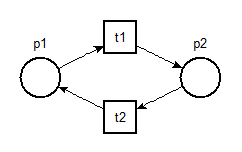
\includegraphics[width=6cm]{./figuras/RDP_SIMPLES.png}\centering
	\fonte{Autoria pr\'opria.}
\end{figure}






Na figura~\ref{fig:esquemaformal} é apresentado uma representa\c{c}\~ao da proposta de desenvolvimento de um projeto, o qual um sistema \'e modelado e ent\~ao a interface, com base na an\'alise do modelo formal, gera um c\'odigo implement\'avel para o controlador selecionado. 

 O esquema est\'a seccionado em sete passos, s\~ao eles:
 
 \begin{itemize}
 	\item Passo 1: Modelagem do sistema f\'isico em Redes de Petri;
 	\item Passo 2: Obten\c{c}\~ao dos aut\^omatos da planta e das especifica\c{c}\~oes;
 	\item Passo 3: Aplica\c{c}\~ao da Teoria de Controle Supervis\'orio;
 	\item Passo 4: Obten\c{c}\~ao do aut\^omato da l\'ogica de controle sintetizada;
 	\item Passo 5: Preparar a l\'ogica de controle para ser convertida;
 	\item Passo 6: Gera\c{c}\~ao do c\'odigo implement\'avel;
 	\item Passo 7: Implementa\c{c}\~ao do c\'odigo em um controlador.
 \end{itemize}

\begin{figure}[!htb]
	%\captionsetup{width=0.97\textwidth}
	\caption[Esquema da abordagem formal para controle de um SED]{Esquema da abordagem formal para controle de um SED.}
	\label{fig:esquemaformal}
	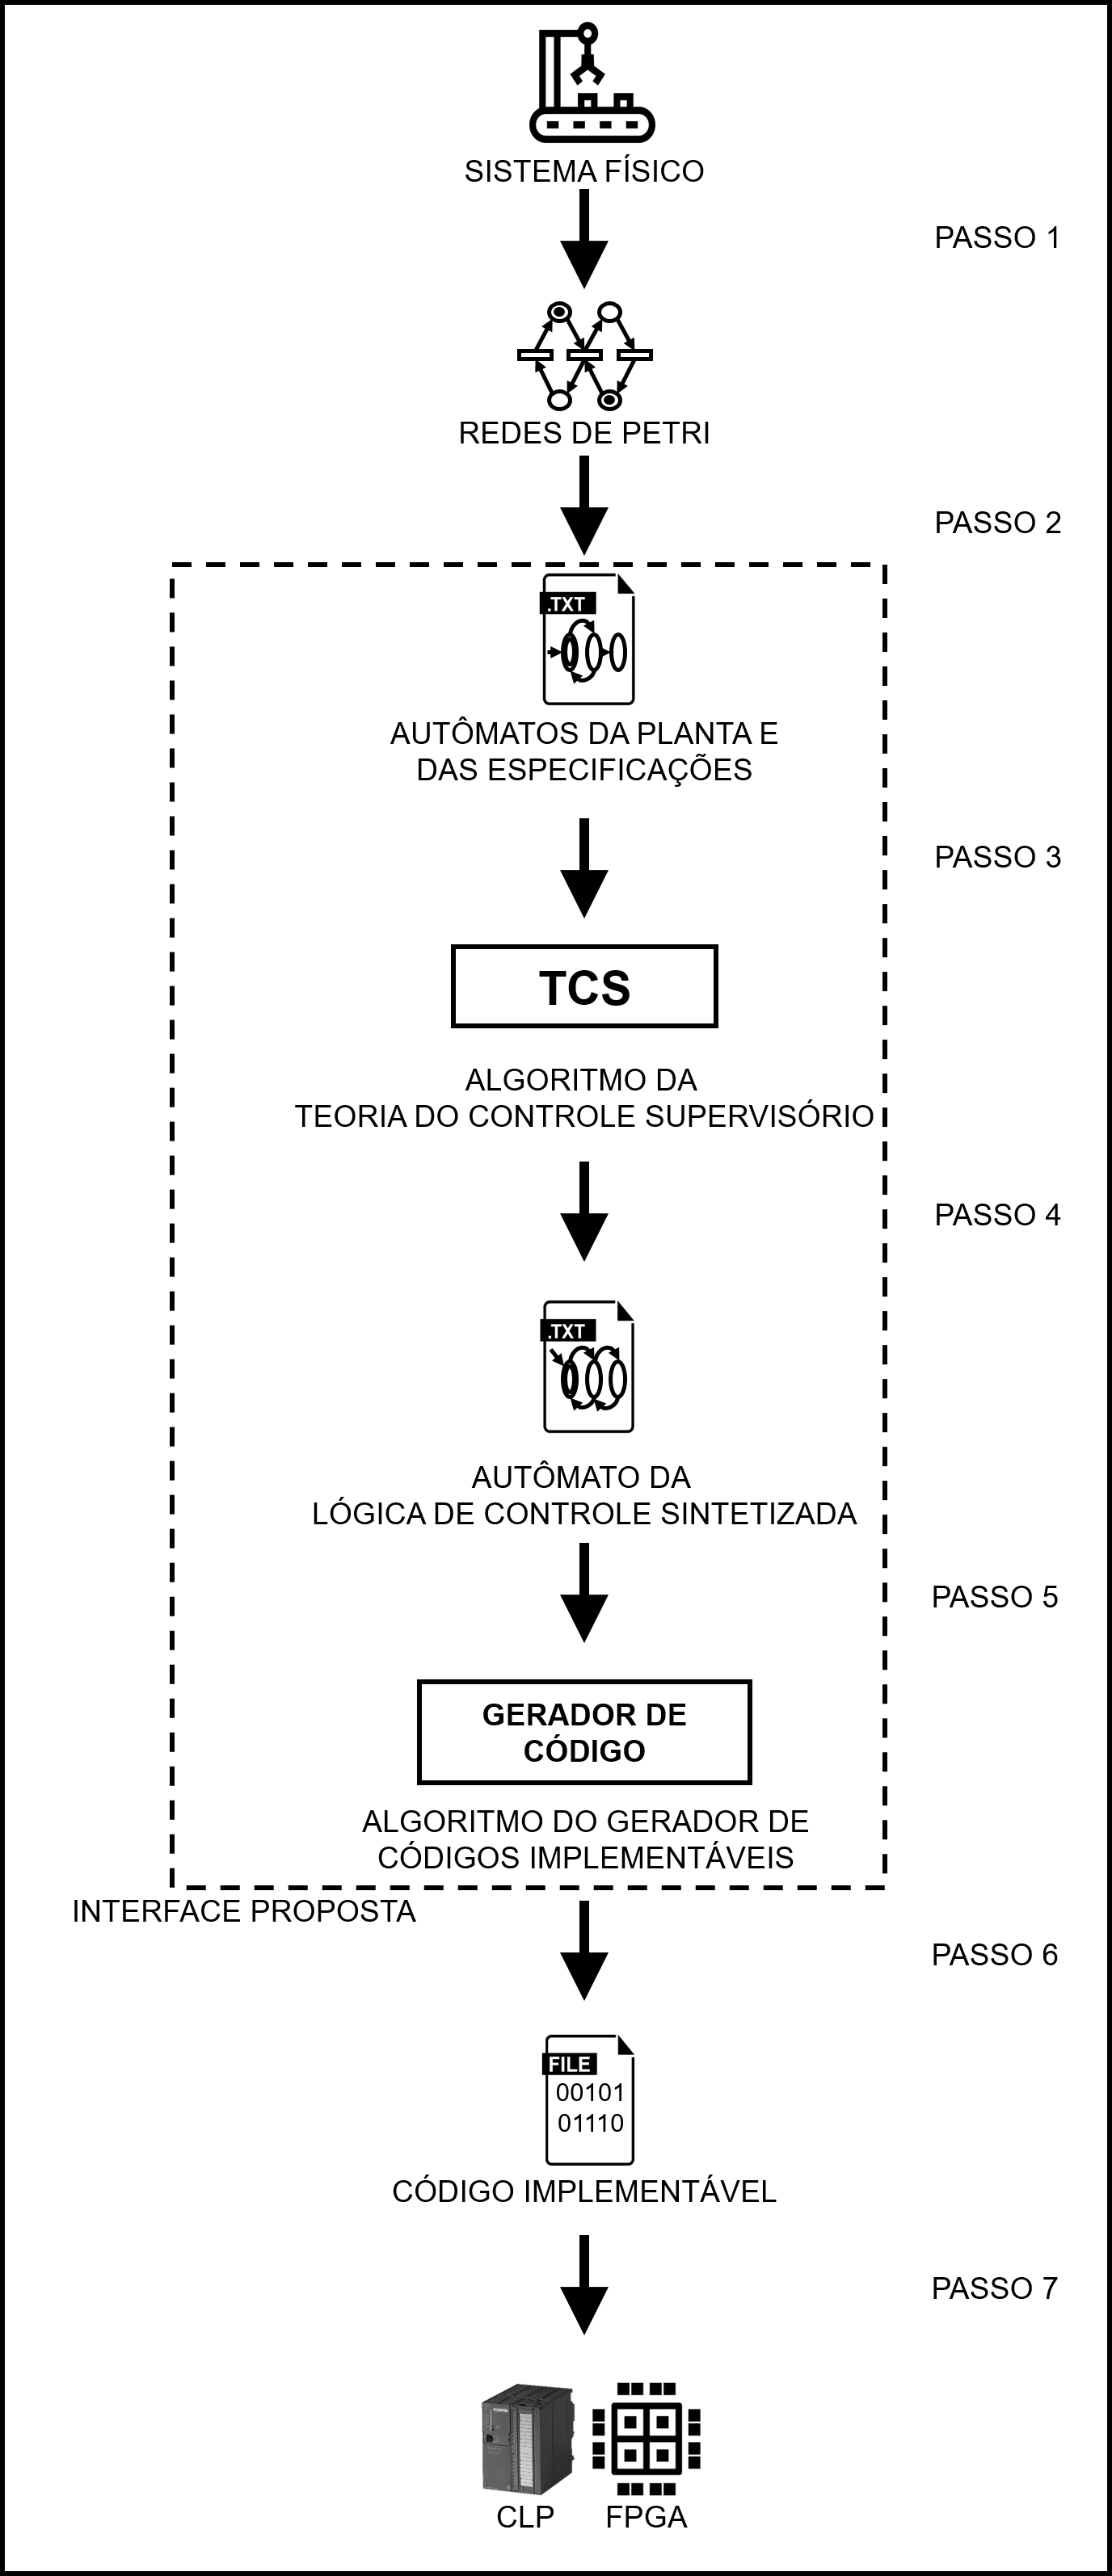
\includegraphics[width=10cm]{./figuras/ESQUEMA_MODELAGEM_FORMAL.png}\centering
	\fonte{Autoria pr\'opria.}
\end{figure}

\subsection{Modelagem do sistema f\'isico em Redes de Petri}


H\'a diversos softwares para modelagem de Redes de Petri, por\'em o software TINA, criado pelo Laborat\'orio de An\'alises e Arquitetura de Sistemas da Universidade de Toulouse, \'e o \'unico que preenche os requisitos para ser executado em conjunto com a interface, gra\c{c}as a formata\c{c}\~ao de seus arquivos de sa\'ida. TINA possui diversas ferramentas para manipular as Redes Petri, tanto para an\'alise quanto para simula\c{c}\~ao. Para este caso a ferramenta de an\'alise de alcan\c{c}abilidade gera para o usu\'ario um arquivo em texto contendo v\'arias informa\c{c}\~oes sobre o grafo de marca\c{c}\~oes.

Neste passo, o usu\'ario modela o sistema f\'isico em Redes de Petri no software TINA.

\subsection{Obten\c{c}\~ao dos aut\^omatos da planta e das especifica\c{c}\~oes}

Uma vez que o sistema foi modelado e analisado, o arquivo oriundo da modelagem do TINA ser\'a carregado na interface, a qual ir\'a rearranjar as informa\c{c}\~oes e dividi-las em m\'aquina de estado finitos devido as marca\c{c}\~oes da rede e demais informa\c{c}\~oes para gerar a especifica\c{c}\~ao do controle supervis\'orio.


\subsection{Aplica\c{c}\~ao da Teoria de Controle Supervis\'orio}

A s\'intese do supervisor \'e realizada para um dado modelo com o objetivo de satisfazer uma especifica\c{c}\~ao de comportamento desejada, onde o supervisor define quais as a\c{c}\~oes de controle que devem ser implementadas \cite{Montgomery2004}.

No caso do algoritmo para aplicar a TCS, se destacam os softwares UMDES \cite{umdes}, desenvolvida pela Universidade de Michigan nos Estados Unidos, e o IDES \cite{ides}, desenvolvida pela Universidade de Queen no Canad\'a. Estes software proporcionam uma f\'acil aplica\c{c}\~ao da TCS partindo de dois aut\^omatos: a planta e as especifica\c{c}\~oes.

\subsection{Obten\c{c}\~ao do aut\^omato da l\'ogica de controle sintetizada}

Neste passo do processo a interface recarrega os aut\^omatos produzidos pelos softwares indicados no item anterior.

\subsection{Preparar a l\'ogica de controle para ser convertida}

A l\'ogica de controle s\'intetizada em forma de aut\^omato \'e formatada para agregar as informa\c{c}\~oes rotuladas durante a modelagem do sistema, essas informa\c{c}\~oes permitem que o c\'odigo a ser gerado contenha os mesmos r\'otulos criado pelo usu\'ario. 

\subsection{Gera\c{c}\~ao do c\'odigo implement\'avel}

A gera\c{c}\~ao dos c\'odigos implement\'aveis ser\'a feita, inspirada nos trabalhos de \cite{hugomestrado} e \cite{disc}, a partir da compara\c{c}\~ao de similaridade da estrutura da l\'ogica sintetizada e a linguagem de programa\c{c}\~ao escolhida.

A programa\c{c}\~ao de controladores l\'ogico program\'aveis em \textit{Sequential Function Chart} (SFC) tem estrutura baseada no \textit{Grafcet}, que por sua vez evoluiu da Redes de Petri, \cite{Martin1999}. Assim, a l\'ogica de controle ser\'a convertida para Redes de Petri e finalmente usada para gerar um arquivo implement\'avel para CLPs em programa\c{c}\~ao SFC.

A gera\c{c}\~ao dos c\'odigos implement\'aveis para FPGAs ser\'a mais simples, pois sua estrutura de programa\c{c}\~ao \textit{VHDL}, uma linguagem de programa\c{c}\~ao de \textit{hardware}, pode ser estruturada como m\'aquina de estados finitos que combina com o aut\^omato sintetizado.

\subsection{Implementa\c{c}\~ao do c\'odigo em um controlador}

O c\'odigo est\'a pronto para ser carregado no controlador selecionado com garantia de controle \'otimo devido ao uso da abordagem formal.

%%%%%%%%%%%%%%%%%%%%%%%



%
%Inserir FIGURA sobre a INTERFACE

%\begin{figure}[!htb]
	%\captionsetup{width=0.97\textwidth}
%	\caption[Esquema dos subsistemas da interface]{Esquema dos subsistemas da interface.}
%	\label{fig:interface}
%	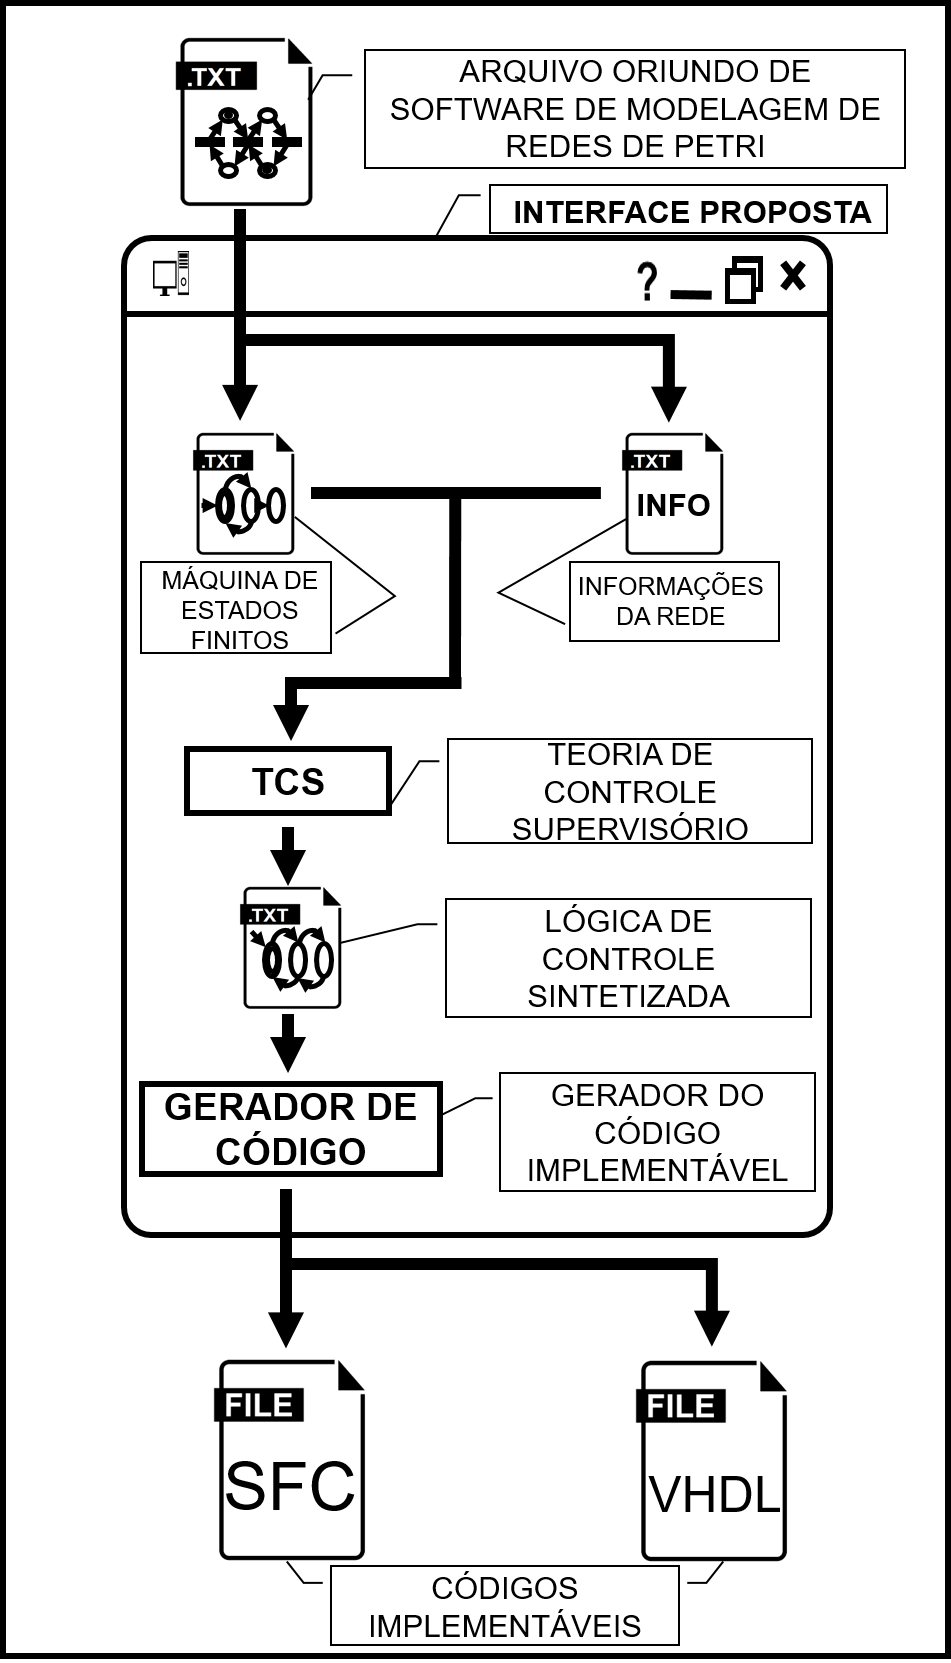
\includegraphics[width=12cm]{./figuras/ESQUEMA_INTERFACE.png}\centering
%	\fonte{Autoria pr\'opria}
%\end{figure}

%H\'a diversos softwares para realizar modelagem e an\'alise de Redes de Petri. Um desses \'e TINA, criado pelo Laborat\'orio de An\'alises e Arquitetura de Sistemas da Universidade de Toulouse. TINA \'e um software de uso livre, e se destaca por possuir uma fun\c{c}\~ao a qual exporta em arquivo de texto as propriedades da rede modelada. Uma das propriedades \'e o grafo, ou \'arvore, de alcan\c{c}abilidade de uma RdP a qual representa todos os estados alcan\c{c}\'aveis e \'e representado por um aut\^omato finito.
%O usu\'ario precisar\'a seguir certas regras ao modelar um sistema, como a rotula\c{c}\~ao de eventos e transi\c{c}\~oes, para que o programa interprete de forma correta as informa\c{c}\~oes. Essas regras estar\~ao presentes na interface do software, bem como um tutorial.

%A partir do grafo de alcan\c{c}abilidade convertido do formato padr\~ao do TINA para o formato de m\'aquina de estados finito, este poder\'a ser executado por outro software para aplicar o Teorema do Controle Supervi\'osio e gerar um aut\^omato supervisor. Entre os softwares que implementam o teorema, se destacam o UMDES, desenvolvida pela Universidade de Michigan, e o IDES, desenvolvida pela Universidade de Queen. A convers\~ao ter\'a base nas informa\c{c}\~oes adicionais, como por exemplo se um evento \'e control\'avel ou somente observ\'avel. O resultado deste processo ser\'a o supervisor do sistema.

%Com o supervisor pronto, o pr\'oximo passo \'e a gera\c{c}\~ao do c\'odigo implement\'avel, este ser\'a realizado seguindo a norma IEC 61131-3, uma norma que rege o padr\~ao de linguagens de programa\c{c}\~ao de controladores l\'ogico program\'aveis, e tamb\'em a norma IEEE 1076, a qual rege a linguagem de descri\c{c}\~ao de hardware VHDL para FPGAs. O programa interpretar\'a o supervisor e ir\'a transcrever este na forma de linhas de c\'odigos. O processo resultar\'a em arquivos pronto para serem embarcados nos sistemas mencionados.



